\chapter{実験の準備}
 提案手法の有効性を検証するため, 実験環境の整備を行った. 本章では, プロセス知識の記述方法の選定から, 指導現場でのインタラクション収集の仕組み, LLMの基礎性能の検証, 実装に至るまでの準備について説明する. 

\section{プロセス知識の記述方法}
本研究では, 西村らが提案したCHARM (Convincing Human Action Rationalized Model) \cite{Nishimura2008, Nishimura2015}を採用する. これは, 人間の行為とその目的を体系的に表現するためのモデルであり, 機械工学分野で用いられる機能分解木の考え方を応用して開発された.

CHARMは,ある行為をそれを達成するために必要な行為の系列に分解することで,行為間の目的達成関係を記述する. 具体的には,上位層の行為ノードを達成するために下位層の行為ノードを実行するという階層構造として表現される. 各ノードには行為の実行者や実行条件などのプロパティを付与することができ,これにより各行為の目的の把握を容易にする. また,同一の目的に対して複数の実現手段が存在する場合,それらを並列的に記述することで,状況に応じた手段の選択を支援する. 

CHARMの重要な特徴として, 形式知化された知識と暗黙知の橋渡しを支援する点が挙げられる. 具体的には, 行為とその目的の関係性を明示することで, 「なぜその行為が必要か」という理由付けを含めた知識表現を実現する. これにより, 単なる手順の羅列ではなく, 状況に応じた柔軟な対応を可能にする知識構造を構築できる.

実際に, 看護業務における技能伝承の現場での実証実験を通じてCHARMの有効性が確認されている. 特に, 暗黙知の抽出や組織間での知識共有においてその有用性が示されている. これは, CHARMが持つ目的指向的な知識表現と問題-対策の構造化という特徴が実践的な知識管理に適していることを示唆している.

本研究では, CHARMを計算機上で扱うためにリレーショナルデータベース(RDB)を構築した(図\ref{fig2}). 実装には木構造をRDBで表現するための閉包テーブルというデータベース構造を採用した.

CHARMに基づいて作成したプロセス知識の例を図\ref{fig3}に示す. これは社交ダンスのナチュラルターンに関するプロセス知識である.

\begin{figure}[htbp]
    \centering
    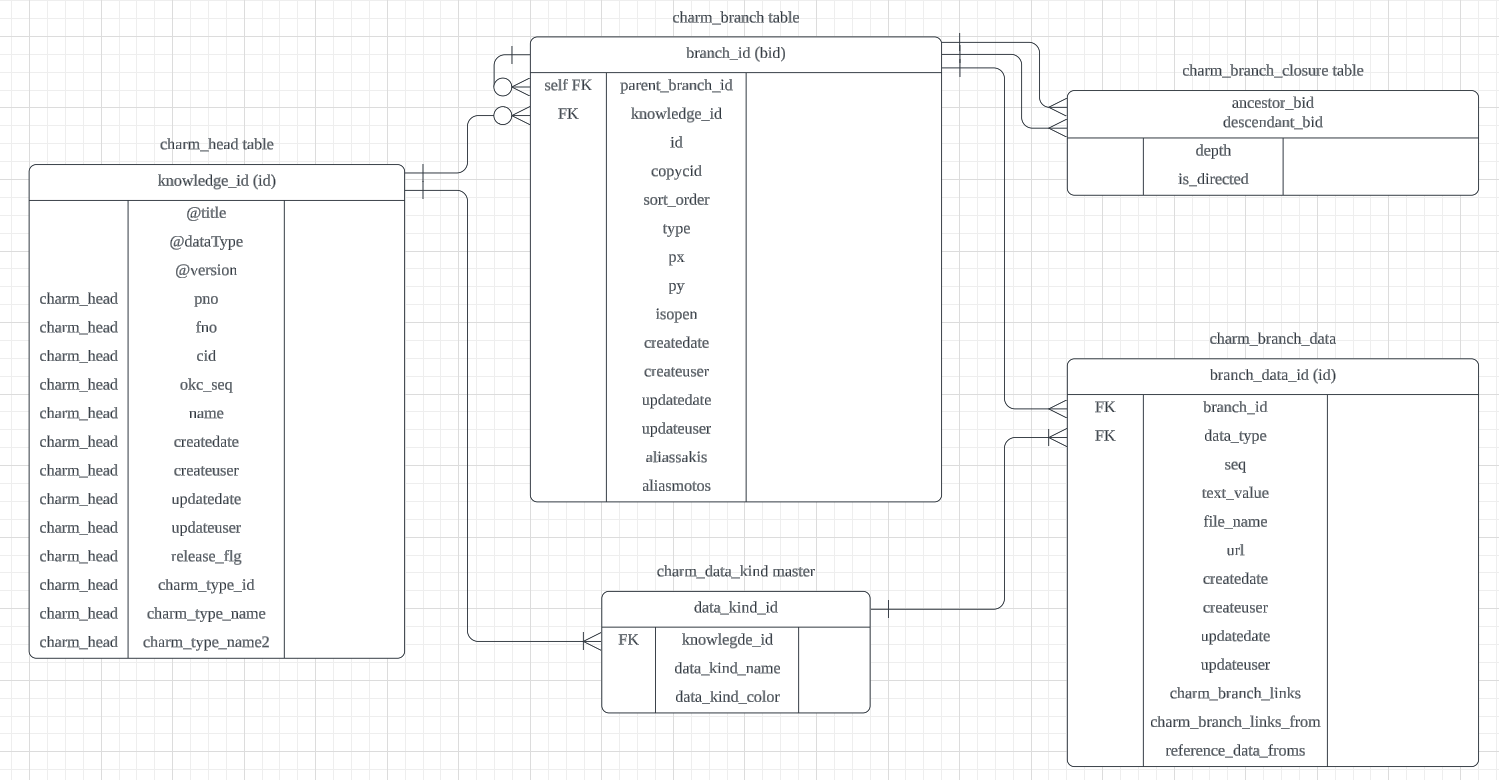
\includegraphics[width=1.0\linewidth]{./image/charm_database.png}
    \caption{CHARMのリレーショナルデータベース表現}
    \label{fig2}
\end{figure}

\begin{figure}[htbp]
    \centering
    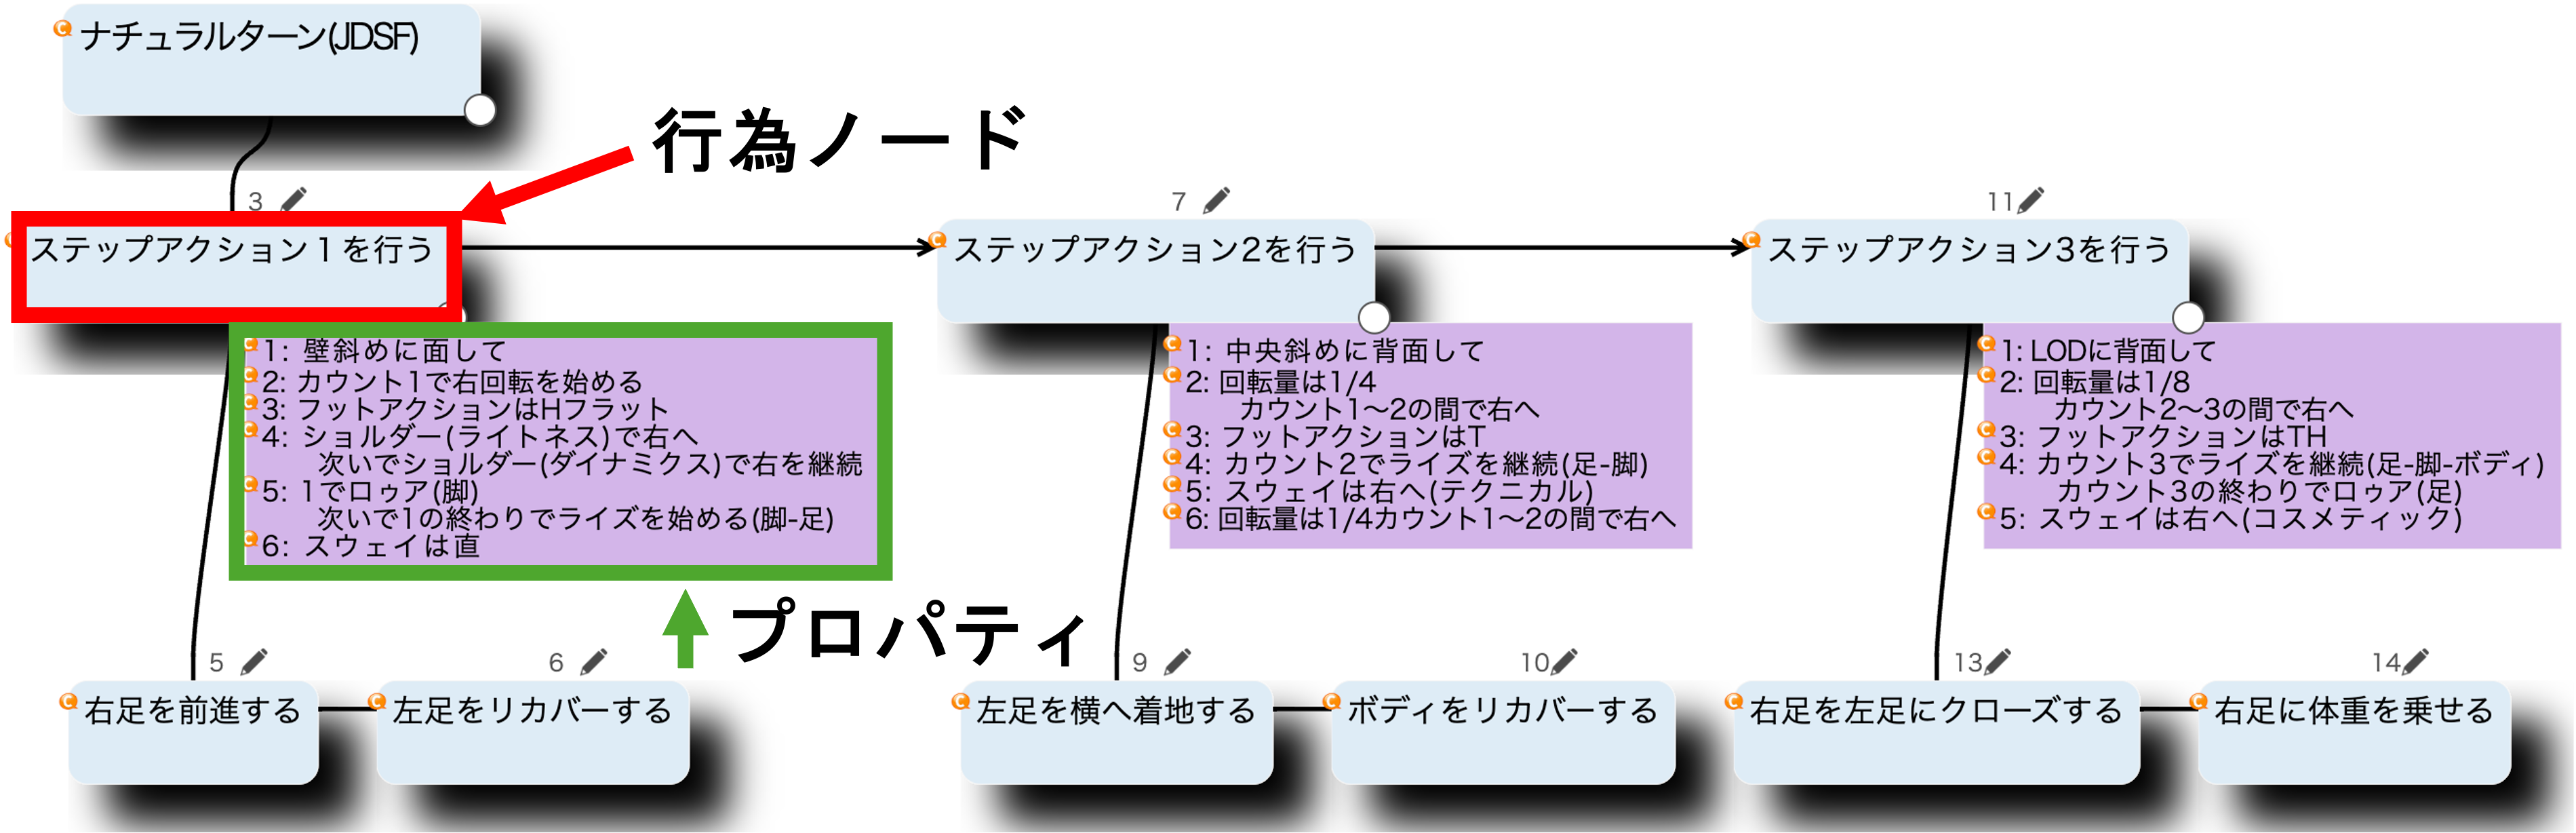
\includegraphics[width=1.0\linewidth]{./image/charm_natural_turn.png}
    \caption{CHARMのリレーショナルデータベース表現}
    \label{fig3}
\end{figure}

\section{指導現場のインタラクションを収集するシステムの開発}


\section{LLMの予備検証とユーザーインターフェイスの開発}
\subsection{モデルの選定}
\subsection{知識抽出における活用可能性の検証}
\subsection{プロンプト及びUIの実装}


 表\ref{table1}が示すように...\\

\begin{table}[h]
    \centering
    \begin{tabular}{r|rr}
    & a & b\\ \hline
    1& 0.25 & 0.33\\
    2& 0.75 & 0.66\\
    \end{tabular}
    \caption{表のキャプション}
    \label{table1}
\end{table}
